\documentclass[11pt]{article}
\usepackage{amsmath}
\usepackage{amsfonts}
\usepackage[margin=1in]{geometry}
\usepackage{graphicx}
\usepackage{amssymb}
\newtheorem{definition}{Definition}
\newtheorem{algorithm}{Algorithm}
\newtheorem{function}{Function}
\graphicspath{{./PNgraph/}}
\begin{document}
\title{Implement Unfolding based POR Algorithm}
\author{Huyen Nguyen}
\date{\today}
\maketitle

\section{Building labelled event structure - parametric semantics}
\subsection{Define the independent relation}
	Find out all pairs of transition commuting at every global state of the net.
	Global state is a marking. 
	\begin{itemize}
	\item compute all reachable markings(already implemented in simple model checker SMC)
	\item Check if transition t is enabled at state s: $check_enabled(t,s)$ (implemented in PNAPI)
	\item Function to check if $t_1$ and $t_2$ commute or not.\\
			check\_commute$(t_1,t_2)$ returns $true$ if $t_1$ and $t_2$ commute and $false$ in reverse.
	\item Call $check\_commute(t_1,t_2)$ for all pairs of transitions, then store all independent pairs in a set
	\end{itemize}

\begin{definition}
	Two transitions t and t' are commuted if:
	\begin{enumerate}
		\item The first condition: If $t, t'\in enable(s) and s\rightarrow ^t s' \Longrightarrow t'\in enable(s')$ 				can be implemented as:
		
		if  $\left( \left((check\_in\_enabl(t,s)\&\& check\_in\_enabl(t',s))\right)
		==check\_in\_enabl(t',fire(s,t)) \right)$
		
		$\qquad$ return true;
		
		$ fire(s,t)$ is a new state reached by firing t at s - function getSuccessor(t) in Marking class
				
		\item If $t, t' \in enable(s) and \exists s": s\xrightarrow{t.t'} s" then s\xrightarrow{t'.t} s"$ 
		
		if $\left(check\_in\_enabl(t,s)\&\& check\_in\_enabl(t',s)\right) == 													\left(fire(fire(s,t),t')==fire(fire(s,t'),t)\right)$
		
	\end{enumerate}
\end{definition}

\subsection{Construct unfolding under the independent relation for a petri net}
	This part details the process of constructing the unfolding (set of prefix) for a petri net under independent 			relation defined in previous section.
	
	Unfolding is a LES, tuple $\varepsilon$ = $\langle E,<,\#,h\rangle$, where E is a set of events, $<$ is set of 			pairs of events in causal relation, $\#$ is set of events in conflict.
	
	\begin{definition}{Construct the unfolding LES}
	
	\begin{enumerate}
		\item Initially, LES having one event $bottom \perp$
		
		\item Let $\varepsilon$ be an prefix containing a history H (one element in the set of possible histories of 				LES) for some transition t $\in$ T.
		
	\end{enumerate}
	\end{definition}


	\begin{function}{Construct unfolding\\}
		Extend() $\backslash\backslash \thickspace \varepsilon$ is a unfolding prefix, initially 								$\varepsilon=\bot$\\
		\{
	
			For each last event (event just added) $e_i$ of $\varepsilon$, do
			
			\texttt{$//$ check only maximal event because all extendable events had already been computed and added 						to the stack \textbf{extendable} in previous step } 
			
			\{	\\
								
			 	For each transition t in transition set
			 		
			 		if ($e_i.getState().activates(t)$)
					
				\qquad if $is\_depend(t, e_i.lbl)==true $
						$//$ can't find $<e_i.lbl,t>$ in independent set
		
					\qquad\qquad make a new Event with $lbl=t$; $his = \{e\_i\}$ to the stack \textbf{extendable} 
					
				\qquad else 	$//$ $<e_i.lbl,t>$ in the set of independent relation
				
						\qquad \{			
						\begin{itemize}
						\renewcommand\labelitemi{-}
							\item \qquad search in set of events of LES, if exists an event $e\_j$ with label t
							\item \qquad compute the 	$state(\sigma)$ with a run $\sigma=t.(e\_i.lbl)$ or 													$(e\_i.lbl).t$
							\item \qquad find all enabled transitions t' at the state.
							\item \qquad Add event $\langle t', \{e_i,e_j\}\rangle$ to the stack \textbf{extendable}
						\end{itemize}
							
						\qquad \}
			
				Pop up an event e from the stack to do: 
				
					\qquad LES.add(e); \textbf{extendable} and add it to LES
						
					\qquad e.computeCfl(); $//$ \texttt{find out all events in conflict with e}
						
					\qquad e.computeState(); $//$ \texttt{compute the marking corresponding to e: 													getSuccessor(e.lbl)}
					
				\}
	
				Call Extend($\varepsilon'$)\\
		\}
\end{function}

	To implement the algorithm, we construct a class Event:
	
	\begin{definition}{Event\\}
		class Event\\
		\{ 
		
		Transition lbl; 	$\backslash\backslash$ the transition labels the event
		
		Config his; 	$\backslash\backslash$ histort: set of all predecessors
		
		set$\langle$Event$\rangle$ cfl;$\backslash\backslash$ set of events conflicting with the event
		
		Marking state;
		
		\textup{public:}
		
		void computeCfl();
		
		bool is\_inHis(Event)
		
		bool enable(Transition);
		
		void setState();\\	
		\}
	\end{definition}
		
\begin{definition}{Configuration} \\
	class Config\\
	\{
	
		set $\langle Event \rangle$  event ; maximal events (no more event which is enabled at them) \\
		\textup{member function:}
		
		Marking computeState();
		
		bool is\_inConfig(Event);
	\}
\end{definition}

\begin{definition}{Labelled Event Structure LES}

	set of history of a prefix $<$
	
	The process of buiding the computation tree:
	
	class LES
	
	\{
	
		set $\langle Event \rangle$ evt;
		
		set $\langle Event,Event \rangle$ causal; not necessary
		
		set $\langle Event,Event \rangle$ conflict; not necessary
	
		Marking computeState
		
	\}
\end{definition}


\begin{function}{Compute set of conflict events in LES}	\\ 
	Function computeCfl(e)\\
	\{\\
	  for all event \textbf{e'} in LES.evt
	  
	  	if $(e'.is\_inHis(e)==false)\&\& ((e.is\_inHis(e')==false)) \&\& is\_depend(e.lbl,e'.lbl)$ 
	  	
	  	then
	  	
	  		add e'to e.cfl;
	  		
	  	end if \\
	  \}
\end{function}	

\begin{function}{Check if t and t'independent} \\
	is\_depend(t,t')\\
	\{
	
		for each pair $(t_1,t_2)$ in independent set
		
		if $(t,t')==(t_1,t_2)$
		
		then return true;\\
	\}		
\end{function}

\begin{function}{Check if event e in History of an event}\\
	is\_inHis(e)\\
	\{
	
		$\backslash*$ return true when e is a event in the calling event.$*\backslash $
	
		for each event $e_i$ in his
	
		if $(e == e_i) $ return true;
	
		return false;\\
	\}	
\end{function}

\begin{function}{Check if t enabled at state of some event}\\
	enable(Transition t)\\
	\{

		$\backslash*$ return true when t is activated at the state of that event.$*\backslash $
	
		return state.activates(t); $\backslash*$ activate(t) is a member function in class Marking $*\backslash $ \\
	\}	
\end{function} 
						
\section{LES exploration}

	Given a prefix unfolding in terms of sets of events like picture attached.

	\begin{figure}
		%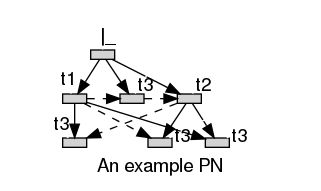
\includegraphics[scale=0.9]{unf.png}
	\end{figure}

	\subsection{Overall algorithm}
		\begin{algorithm}{POR exploration algorithm} \\
			\textup{Procedure Explore(C,D,A)} \\
			\{	
					
				\textup{Extend(C)}
				
				\let\emptyset\varnothing
				if $ en(C) = \emptyset $  return
				
				if $A=\emptyset$
		
					\textup{Choose e from en(C)}
				
				else
				
					 e form $A\cap en(C)$
					
				\textup{Explore($C\cup\{e\},D,A\setminus\{e\}$ )}
				
				If $\exists J \in Alt(C,D\cup\{e\})$
				
				$Explore(C,D\cup\{e\},J\setminus C)$
				
				\textup{Remove(e,C,D)}\\
			\}
			
		\end{algorithm}
		
	\subsubsection{A configuration}
		- Check if a set of events is a configuration is\_config()\\
		\textit{A configuration is a set of events that are causally closed and conflict free.}
		
		
		\subsubsection{Compute en(C)}
		Compute a set of events enabled at a given configuration C
\end{document}
